\documentclass[a4paper,12pt]{article}
\usepackage{graphicx}
\usepackage{xcolor}
\usepackage{fancyhdr}
\pagestyle{fancy}
\fancyhead[L]{Peter Maina}
\fancyhead[R]{September 6, 2024}

\title{HOST DISCOVERY}
\author{Peter Maina}
\date{\today}

\begin{document}

\maketitle

\section{Host Discovery}

We have created a virtual box of a Windows 11 OS (VICTIM) and bridged our Ethernet connection to the box.
\begin{figure}[h]
    \centering
    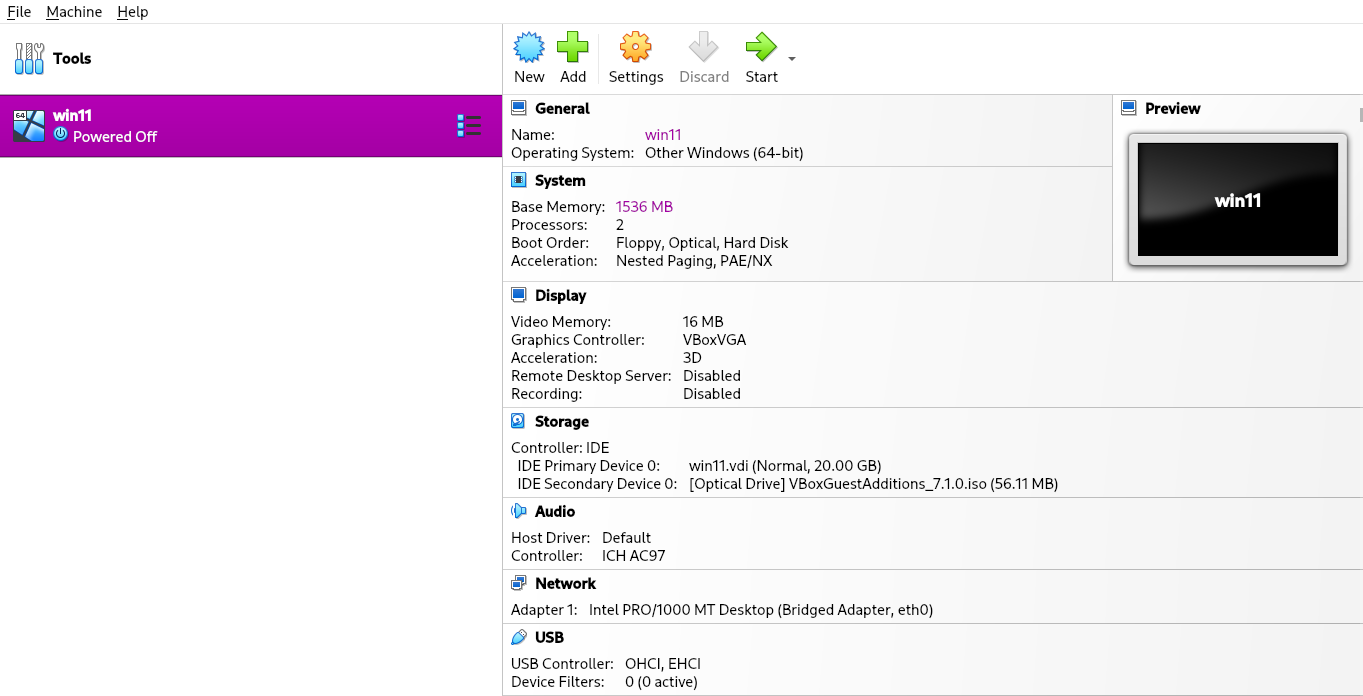
\includegraphics[width=0.8\textwidth]{vm.png}
    \caption{Virtual Machine Setup}
    \label{fig:vm_setup}
\end{figure}

The host machine is a KALI LINUX machine (ATTACKER). We own both systems and we are using our network for any penetration testing.

From our KALI we will try to discover the victim machine's IP address. Since the victim is using the same network as the host, we will first discover our own IP.

\subsection{Discovering Our Own IP Address}

\begin{verbatim}
ifconfig
\end{verbatim}

\begin{verbatim}
eth0: flags=4163<UP,BROADCAST,RUNNING,MULTICAST>  mtu 1500
        inet 192.168.0.101  netmask 255.255.255.0  broadcast 192.168.0.255
        inet6 fe80::2e59:e5ff:feba:4e62  prefixlen 64  scopeid 0x20<link>
        ether 2c:59:e5:ba:4e:62  txqueuelen 1000  (Ethernet)
        RX packets 12070  bytes 8155689 (7.7 MiB)
        RX errors 0  dropped 37  overruns 0  frame 0
        TX packets 11677  bytes 2074242 (1.9 MiB)
        TX errors 0  dropped 0 overruns 0  carrier 0  collisions 0
        device interrupt 17  memory 0xd4400000-d4420000  

lo: flags=73<UP,LOOPBACK,RUNNING>  mtu 65536
        inet 127.0.0.1  netmask 255.0.0.0
        inet6 ::1  prefixlen 128  scopeid 0x10<host>
        loop  txqueuelen 1000  (Local Loopback)
        RX packets 68  bytes 3878 (3.7 KiB)
        RX errors 0  dropped 0  overruns 0  frame 0
        TX packets 68  bytes 3878 (3.7 KiB)
        TX errors 0  dropped 0 overruns 0  carrier 0  collisions 0

wlan0: flags=4163<UP,BROADCAST,RUNNING,MULTICAST>  mtu 1500
        inet 192.168.0.102  netmask 255.255.255.0  broadcast 192.168.0.255
        inet6 fe80::d6cf:98b5:4b4c:8225  prefixlen 64  scopeid 0x20<link>
        ether 6c:88:14:18:88:60  txqueuelen 1000  (Ethernet)
        RX packets 203  bytes 35256 (34.4 KiB)
        RX errors 0  dropped 0  overruns 0  frame 0
        TX packets 43  bytes 17536 (17.1 KiB)
        TX errors 0  dropped 0 overruns 0  carrier 0  collisions 0

\end{verbatim}

We will need the Ethernet (\texttt{eth0}) IP.

We can use a tool called \texttt{ipcalc} to see the IP subnet mask range of 192.168.215.......

\begin{verbatim}
ipcalc 192.168.0.101
\end{verbatim}

\begin{verbatim}
ipcalc 192.168.0.101
Address:   192.168.0.101        11000000.10101000.00000000. 01100101
Netmask:   255.255.255.0 = 24   11111111.11111111.11111111. 00000000
Wildcard:  0.0.0.255            00000000.00000000.00000000. 11111111
=>
Network:   192.168.0.0/24       11000000.10101000.00000000. 00000000
HostMin:   192.168.0.1          11000000.10101000.00000000. 00000001
HostMax:   192.168.0.254        11000000.10101000.00000000. 11111110
Broadcast: 192.168.0.255        11000000.10101000.00000000. 11111111
Hosts/Net: 254                   Class C, Private Internet

\end{verbatim}

From the output, the subnet mask seems to be 24.

\subsubsection{Given IP Address}
The IP address analyzed is:

\[
\text{192.168.0.101}
\]

In binary notation:

\[
\text{192.168.0.101} = 11000000.10101000.00000000.01100101
\]

\subsubsection{Subnet Mask}
The subnet mask provided is:

\[
\text{255.255.255.0}
\]

In binary:

\[
\text{255.255.255.0} = 11111111.11111111.11111111.00000000
\]

This corresponds to a \textbf{CIDR (Classless Inter-Domain Routing)} notation of:

\[
/24
\]

\subsubsection{Wildcard Mask}
The wildcard mask is the inverse of the subnet mask:

\[
\text{0.0.0.255}
\]

In binary:

\[
00000000.00000000.00000000.11111111
\]

This is commonly used in Access Control Lists (ACLs) and firewall rules.

\subsubsection{Network Address}
The \textbf{network address} is obtained by performing a bitwise AND between the IP address and the subnet mask:

\[
\text{192.168.0.101} \land \text{255.255.255.0} = \text{192.168.0.0}
\]

In binary:

\[
\text{11000000.10101000.00000000.01100101} \land 
\text{11111111.11111111.11111111.00000000} =
\text{11000000.10101000.00000000.00000000}
\]

Thus, the network address is:

\[
\textbf{192.168.0.0/24}
\]

\subsubsection{Usable Host Range}
The first and last usable IP addresses within the network are:

- \textbf{Minimum Host Address} (First usable IP):
  
  \[
  \text{192.168.0.1}
  \]

  \[
  \text{11000000.10101000.00000000.00000001}
  \]

- \textbf{Maximum Host Address} (Last usable IP):

  \[
  \text{192.168.0.254}
  \]

  \[
  \text{11000000.10101000.00000000.11111110}
  \]

\subsubsection{Broadcast Address}
The \textbf{broadcast address} is found by setting all host bits to 1:

\[
\text{192.168.0.255}
\]

In binary:

\[
\text{11000000.10101000.00000000.11111111}
\]

This address is used to send packets to all hosts in the subnet.

\subsubsection{Total Usable Hosts}
The number of usable hosts is calculated as:

\[
2^h - 2
\]

where \( h \) is the number of host bits. Since a /24 subnet has \( 8 \) host bits:

\[
2^8 - 2 = 256 - 2 = 254
\]

The subtraction of 2 accounts for:

1. The network address (\textbf{192.168.0.0}).
2. The broadcast address (\textbf{192.168.0.255}).

Thus, the subnet allows for \textbf{254 usable host addresses}.

\subsubsection{Class and Private Network}
- The IP address \textbf{192.168.0.101} belongs to \textbf{Class C}.
- IP range for Class C: \( 192.0.0.0 \) to \( 223.255.255.255 \).
- Default subnet mask for Class C: \( 255.255.255.0 \).
- The address falls within the \textbf{private IP range} (RFC 1918), meaning it is not routable on the public internet.


\subsection{Using Nmap}

\begin{verbatim}
sudo nmap -PE -sn 192.168.0.0/24 -oN hostdiscovery.txt
\end{verbatim}

\begin{verbatim}
        Starting Nmap 7.95 ( https://nmap.org ) at 2025-03-21 07:07 EDT
        Nmap scan report for 192.168.0.1
        Host is up (0.00072s latency).
        MAC Address: C8:3A:35:50:0D:C0 (Tenda Technology)
        Nmap scan report for 192.168.0.104
        Host is up (0.00026s latency).
        MAC Address: 08:00:27:DC:BC:E6 (PCS Systemtechnik/Oracle VirtualBox virtual NIC)
        Nmap scan report for 192.168.0.101
        Host is up.
        Nmap done: 256 IP addresses (3 hosts up) scanned in 2.59 seconds
        
\end{verbatim}

From the output, we have 3 hosts discovered, and our target is given as \texttt{192.168.215.50}. Since it is hosted on the VirtualBox, the rest are our network source and the local machine (KALI).

We have successfully identified our host using NMAP.

\subsection{Using Bettercap}

Bettercap is a network discovery and sniffing tool that can sniff on devices connected to our network, so it can do more than host discovery.
By comparing the Nmap results 192.168.0.104 have a common vender "PCS Systemtechnik GmbH " which takes the virtualbox place making it our target.

\begin{verbatim}
[sudo] password for eclipse: 
bettercap v2.33.0 (built for linux amd64 with go1.22.6) [type 'help' for a list of commands]

192.168.0.0/24 > 192.168.0.101  » [07:08:37] [sys.log] [inf] gateway monitor started ...
192.168.0.0/24 > 192.168.0.101  » net.probe on
[07:08:45] [sys.log] [inf] net.probe starting net.recon as a requirement for net.probe
[07:08:45] [endpoint.new] endpoint 192.168.0.104 detected as 08:00:27:dc:bc:e6 (PCS Systemtechnik GmbH).
192.168.0.0/24 > 192.168.0.101  » [07:08:45] [sys.log] [inf] net.probe probing 256 addresses on 192.168.0.0/24
192.168.0.0/24 > 192.168.0.101  » net.[07:08:48] [endpoint.new] endpoint 192.168.0.100 detected as 6a:9c:b6:d2:7b:6e.
192.168.0.0/24 > 192.168.0.101  » net.show

┌───────────────┬───────────────────┬─────────┬────────────────────────────┬───────┬───────┬──────────┐
│     IP ▴      │        MAC        │  Name   │           Vendor           │ Sent  │ Recvd │   Seen   │
├───────────────┼───────────────────┼─────────┼────────────────────────────┼───────┼───────┼──────────┤
│ 192.168.0.101 │ 2c:59:e5:ba:4e:62 │ eth0    │ Hewlett Packard            │ 0 B   │ 0 B   │ 07:08:37 │
│ 192.168.0.1   │ c8:3a:35:50:0d:c0 │ gateway │ Tenda Technology Co., Ltd. │ 172 B │ 172 B │ 07:08:37 │
│               │                   │         │                            │       │       │          │
│ 192.168.0.100 │ 6a:9c:b6:d2:7b:6e │         │                            │ 120 B │ 92 B  │ 07:08:48 │
│ 192.168.0.104 │ 08:00:27:dc:bc:e6 │         │ PCS Systemtechnik GmbH     │ 0 B   │ 92 B  │ 07:08:45 │
└───────────────┴───────────────────┴─────────┴────────────────────────────┴───────┴───────┴──────────┘

↑ 14 kB / ↓ 36 kB / 798 pkts

\end{verbatim}

From Bettercap, we can see our hosts but we can't tell the target's IP. Since we have a fewer number of hosts, we can eliminate our local machine and/or network gateway. Bettercap also gave us the target's name as \texttt{ADMIN.connectify}, which can be used for further attacks.

\section{Conclusion}

From this, we have successfully performed host discovery using two tools.

\newpage{}
\section{further Info Gathering using NMAP}
Since our host is up and running; which we can always check by pinging target;but our pings might be blocked by windows firewall
that blocks ICMP pings for security reasons.
\begin{verbatim}
        ping 192.168.0.104
PING 192.168.0.104 (192.168.0.104) 56(84) bytes of data.
^C
--- 192.168.0.104 ping statistics ---
4 packets transmitted, 0 received, 100% packet loss, time 3054ms

\end{verbatim}
We can use Nmap to see the services running on the target and the version of the services; NMAP can be very important at this stage 
to know more about the target.

\end{document}
